\documentclass[12pt,a4paper]{article}
\usepackage[utf8]{inputenc}
\usepackage[sfdefault]{roboto}
\usepackage[T1]{fontenc}
\usepackage{xcolor}
\usepackage{amsmath}
\usepackage{amsfonts}
\usepackage{amssymb}
\usepackage[ngerman]{babel}
\usepackage{amssymb}
\usepackage{microtype}
\usepackage{wrapfig}
\usepackage[left=2.5cm,right=2cm,top=2cm,bottom=2cm]{geometry}
\usepackage{graphicx}

\begin{document}

\begin{titlepage}
\title{\vspace*{1cm} \huge{\textbf{SVM - Outdoor}} \\ \textbf{Webprojekt 2019}\\
\vspace*{2cm}
\begin{figure}[htb]
\advance\leftskip-2cm

\includegraphics[scale=1.2]{Startseite.png}
\end{figure}
\vspace{2cm}}
\author{\textbf{Enrico Bachus, Urs Egenberger, Lisa Fremdt, Leonie Knödler,}\\ \textbf{Tomas Kostadinov, Dominik Ruf}}
\date{\vspace{2cm} \textbf{9.12.2019}}

\end{titlepage}
\maketitle
\newpage
\tableofcontents
\newpage


\section{Thema}
Als erste Projektarbeit an der Dualen Hochschule, bekamen wir die Aufgabe eine Website für den Sportverein SVM zu bauen. Der Kurs A bekam dabei die Abteilung \dq Outdoor\dq \ zugeteilt. 
\begin{wrapfigure}{r}{5.5cm}
  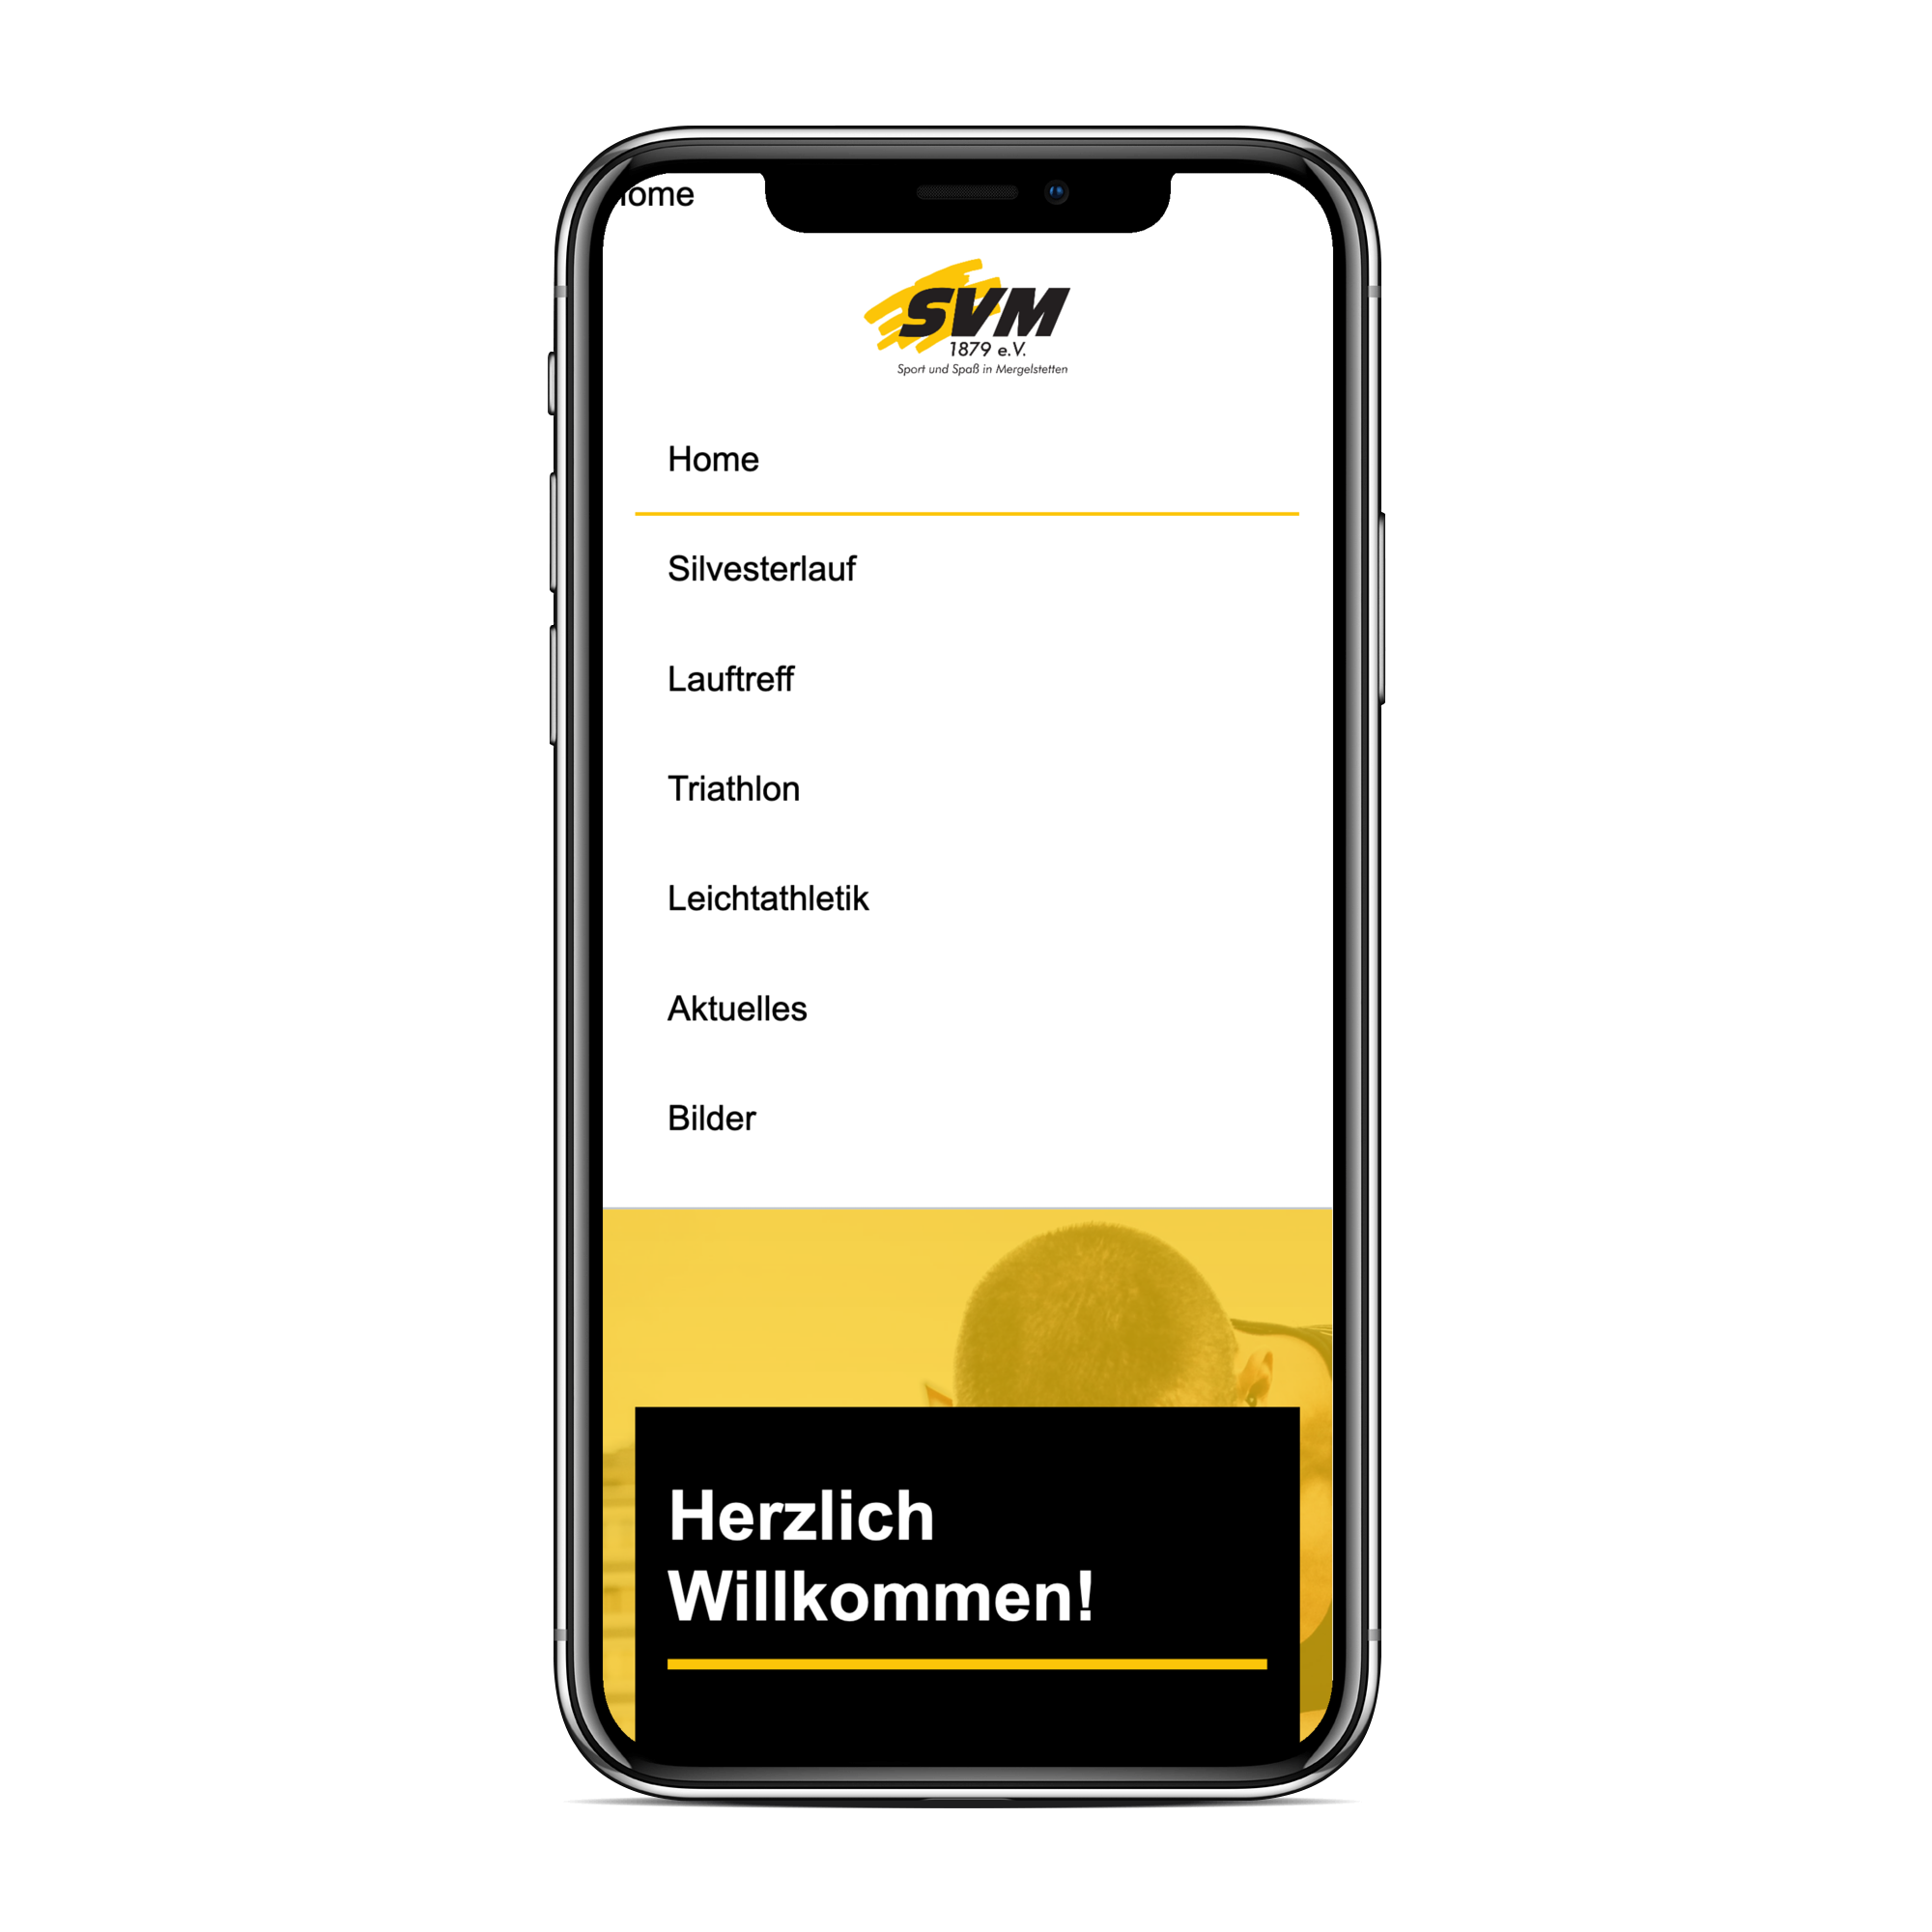
\includegraphics[width=5cm]{iphone.png}
  \caption{Mobile Ansicht}
\end{wrapfigure}
Dafür, um allen Anforderungen gerecht werden zu können, haben wir ein Lastenheft bekommen. 
Hierin sind alle Anforderungen seitens des Vereins, beziehungsweise der Abteilung, an die Webseite enthalten.\\
Da die Abteilung aus mehreren Bereichen besteht, war es klar, dass unsere Website einige Unterseiten enthalten wird. Die Seite \dq Home\dq \ ist die größte, mit insgesamt fünf weiteren Unterseiten. Als nächstes folgt die Seite \dq Silvesterlauf\dq \ diese enthält weitere Unterseiten wie unter anderem eine Ausschreibung, Anmeldung und Ergebnisse. Die Abteilung enthält auch einen Lauftreff, diese Seite enthält weitere drei Unterseiten. Der SVM bietet auch Triathlon-Training an, diese Seite enthält ebenfalls drei Unterseiten. Die fünfte Seite ist die Leichtathletik, diese bietet wie Triathlon und Lauftreff ebenfalls drei Unterseiten.\\
Da Aktuelles auf keiner Website eines Sportvereins fehlen darf, wird auch eine Seite für aktuelle Events und wichtige Informationen entstehen. 
Um auch Bildern einen geeigneten Bereich zu geben, wird es auch eine Bildergalerie geben, in welcher die Besucher der Website die Möglichkeit haben, Bilder von Events, Läufen und Feiern zu betrachten. \\
Da die Website auch dem Leiterteam nutzen soll, wird es auch eine Seite \dq Intern\dq \ geben, in welchem die Trainer die Möglichkeit haben die Finanzen einzusehen, sowie Protokolle und verschiedenen Journals zu hinterlegen. 
\section{Organisation}
Unsere Gruppe war schnell gefunden. Nun aber standen wir vor vielen Fragen: Wie gehen wir an die Aufgabe heran? Worauf legen wir viel Wert? Was ist uns nicht so wichtig?\\ 
Zum Glück waren wir uns in den meisten Fragen einig. Da wir alle unterschiedlich praktische Erfahrungen mit Webprogrammierung und Webdesign hatten, ergänzten wir uns in der Gruppe sehr gut. \\
Es war auch von Anfang an klar, dass wir mit Arbeitsteilung an die Aufgabe heran gehen. Da Arbeitsteilung die schnellste und effektivste Art ist, eine Gruppenarbeit zu bearbeiten, schien uns diese Art am sinnvollsten. Dennoch war es uns sehr wichtig, dass jedes Mitglied der Gruppe einen exakten Überblick darüber hat, wie weit wir sind, was wir machen und vor allem was gemacht wird. Jeder hatte zum Ziel etwas aus der Gruppenarbeit zu lernen. Sei es mehr Erfahrung und mehr Können in der Webprogrammierung, oder einfach nur die Art und Weise wie man eine Gruppenarbeit strukturiert und anpackt. \\
Unsere Arbeitsteilung sah in etwa wie folgt aus: Der Erfahrenste unserer Gruppe hat uns erst einmal erklärt, wie wir an die Programmierung herangehen, sprich womit man am Besten beginnt und womit man bis zum Schluss wartet. Weitere Gruppenmitglieder haben sich Gedanken über das Layout unserer Website gemacht. Ein weiteres Mitglied hat die Rolle des Protokolllisten übernommen. Er hat dokumentiert, wann wir was gemacht haben, damit wir später für die Dokumentation viel Material haben. \\
Trotz Arbeitsteilung haben wir jedem den Freiraum und die Möglichkeit gelassen, in anderen Bereichen mitzuwirken. Alle Ideen und Vorschläge wurden angehört, diskutiert und später eben realisiert oder aus verschiedenen Gründen, wie Zeitaspekt oder Grad der Wichtigkeit weggelassen. \\
Mit regelmäßigen Treffen und dank GitHub, was später näher beleuchtet wird, wusste jeder immer ganz genau darüber Bescheid, wie weit wir sind und was verändert wurde. Bei diesen Treffen wurden Unklarheiten, zum Beispiel in Bezug auf den Quelltext, aufgeklärt und Fortschritte erklärt. Es wurden auch viele Fragen beantwortet und die Fortgeschrittenen unserer Gruppe, haben sich viel Zeit genommen, um den Einsteigern viel über die Webprogrammierung bei zu bringen. Deshalb können wir auch gewährleisten, dass jedes Mitglied für die Erstellung von mindestens zwei Unterseiten unserer Website zuständig war. Dadurch haben alle einige Skills in der Programmierung dazu gewonnen und jeder hat an der Realisierung der Website mitgewirkt.\\
\subsection{Projektmanagement}
Beim \dq Startschuss\dq \, dem sogenannten Kick-Off-Meeting, unserer Projektarbeit, wurden uns die drei verschiedenen Ansätze des Projektmanagements vorgestellt: der klassische, der agile und der hybride Ansatz.\\
Für unsere Projektarbeit haben wir uns, entsprechend der Vorgabe, für das hybride Projektmanagement entschieden, das eine Kombination aus dem agilen und klassischen Projektmanagement darstellt. Hierbei wird die klare Gliederung in Projektphasen aus dem klassischen Projektmanagement übernommen und mit agilen Ansätzen innerhalb der einzelnen Projektphasen verbunden. Die Zwischenergebnisse sollen außerdem präsentiert und Anforderungen gegebenenfalls adaptiert werden. \\
Wie genau wir den hybriden Ansatz in unsere Projektarbeit integriert haben, zeigt sich in unserem Projektplan.

\subsubsection{Projektplan}
\begin{figure}[!htbp]
\advance\rightskip-1cm
	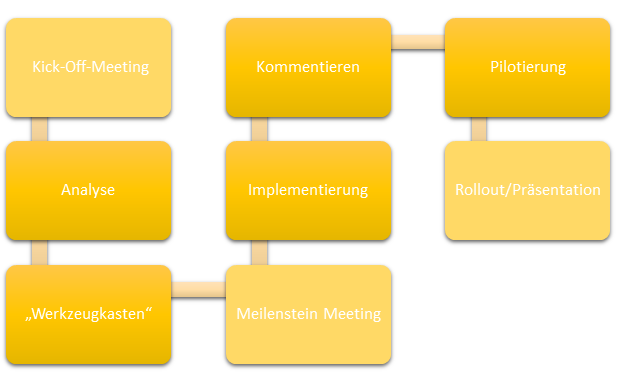
\includegraphics[scale=1.25]{Projektablauf.png}
	\caption{Projektplan}
	\label{img:Projektplan}
\end{figure}

\paragraph{Kickoff-Meeting}
Beim \textit{Kick-Off-Meeting} bekommen wir eine kleine  Einführung in die Thematik, Informationen zum Ablauf der Projektarbeit, die Aufgabenstellung für dieses Semester und das Lastenheft als Grundlage für unsere Arbeit.
\paragraph{Analyse}
Die erste Phase, in der wir selbst etwas erarbeiten, stellt die \textit{Analyse} der Projektaufgabe dar. Sie beinhaltet das Sammeln von ersten Ideen und  die Besprechung der Vorgehensweise in Abhängigkeit von der Aufgabenstellung.
\paragraph{Werkzeugkasten}
In der dritten Phase des Projektplans bauen wir einen sogenannten \textit{Werkzeugkasten}. Der Werkzeugkasten ist ein HTML-Dokument, in dem wir unsere Grundbausteine der Webseite definieren.
\paragraph{Meilenstein Meeting}
Das \textit{Meilenstein-Meeting} stellt eine Möglichkeit dar, unseren Projektplan, sowie den aktuellen Stand bis dahin zu präsentieren und Fragen zu stellen, damit keine Missverständnisse auftauchen und unsere Projektarbeit sich nach Zufriedenheit beider Parteien (sowohl unserer Gruppe, als auch der Projektleiterin) entwickelt.
\paragraph{Implementierung}
Die \textit{Implementierung} beschreibt das Einbauen von Strukturen in das System und umfasst den größten Zeitaufwand.
\paragraph{Kommentieren}
Beim \textit{Kommentieren} wird der HTML-Quelltext mit Kommentaren versehen, sodass er auch für alle weiteren Personen, die mit der Webseite arbeiten werden, verständlich ist.
\paragraph{Pilotieren}
Die letzte Phase vor der endgültigen Abgabe unserer Projektarbeit ist die \textit{Pilotierung}. Hierbei wird die Website auf eine einwandfreie Funktionalität in allen gängigen Webbrowsern,  die Nutzerfreundlichkeit, sowie die Änderbarkeit und Wartungsfähigkeit getestet.
\paragraph{Rollout/Präsentation}
Beim sogenannten \textit{Rollout}, unserer Abschlusspräsentation im ersten Semester, stellen wir dann endlich unser Ergebnis vor.
\subsubsection{Zeitplan}
Unser Ziel hinsichtlich des Zeitmanagements ist uns schon seit Beginn unserer Projektarbeit klar: 
Wir wollen so schnell wie möglich die Website fertigstellen, damit die Projektarbeit so wenig wie möglich bzw. nicht mit dem Prüfungsstress gegen Ende des Semesters zusammenfällt.
Demnach haben wir schon relativ früh mit unseren Gruppentreffen und somit der Arbeit am Projekt gestartet. In der nachfolgenden Tabelle sind all unsere Treffen aufgelistet, in denen wir gemeinsam am Projekt gearbeitet und unsere bisherigen Ansätze aufeinander abgestimmt haben. Ab dem genannten 27. Oktober bis zum 22. November hat jedes Teammitglied seine zugeteilten Unterseiten erstellt und mit Inhalt gefüllt. \\
\begin{table}
\begin{tabular}[h]{c|c|p{9cm}}
\hline
\textbf{Termin} & \textbf{Aktivität} & \textbf{Beschreibung} \\
\hline
7. Oktober & Kick-Off-Meeting & Wir haben uns in einer Gruppe zusammengefunden, einen Gruppennamen ausgedacht und einen Teamleader bestimmt. \\
\hline
16. Oktober & Gruppentreffen & Bei unserem zweiten Treffen lag die Erstellung der ersten Skizzen unserer Website und die
Besprechung der groben Struktur im Fokus. Dabei haben wir den Farbrahmen festgelegt. Am gleichen Tag haben wir bei einem weiteren Treffen die HTML Grundstruktur erstellt. Hierbei ging es darum, Webelemente in einer HTML Sammeldatei zusammenzufassen, so dass bei der Erstellung der Website jeder das gleiche Design verwendet.  Beispiele hierfür sind die Metadaten, der Header, die Navigation, Buttons, der Footer, Checkboxen, Heros (Titelbildboxen)etc.\\
\hline
20. Oktober & Gruppentreffen & Um an einer zentralen Stelle an diesem Projekt arbeiten zu können haben wir Github in der Gruppe eingeführt. Dazu erfolgte eine kleine Einweisung in dem Sinne, dass jeder die zuvor aufgeteilten Unterseiten als Branch erstellt (z.B. import/triathlon – import, um zu verdeutlichen, dass es eine neue Seite ist die hinzugefügt werden soll und dahinter deren Name).
Zum Ende des Treffens haben wir noch kleinere Anpassungen an unserer Grundstruktur gemacht.\\
\hline
27. Oktober & Gruppentreffen & Ziel des Treffens war es alle Unterseiten nun auf die Mitglieder aufzuteilen, sowie Metadaten von Social Media Plattformen wie Twitter und Facebook hinzuzufügen, so dass die Einbindung unserer Website bei den entsprechenden Portalen gut funktioniert. Als letzten Schwerpunkt an diesem Meeting hatten wir die Erstellung der Präsentation für das Meilensteinmeeting.\\
\hline
30. Oktober & Meilenstein Meeting & Wir haben unser Vorgehen und unsere Website vorgestellt.\\
\hline
22. November & Gruppentreffen & Bei diesem Treffen haben wir die letzten ToDos der Website und Dokumentationsaufgaben aufgeteilt. Darunter sind z.B. Optimierungen wie Bilder Komprimierung und das Herunterladen der extern eingebundenen Bilder gefallen. Weiter haben wir letzte Designanpassungen besprochen. \\
\hline
09. Dezember & \multicolumn{2}{c}{Ergebnis Präsentation und Abgabe} \\
\hline

\end{tabular}
\caption{Ablauf}
\label{table:Ablauf}
\end{table}

\newpage
\section{Aufbau und Struktur}
\subsection{Erste Skizzen}
\begin{figure}[!htbp]
	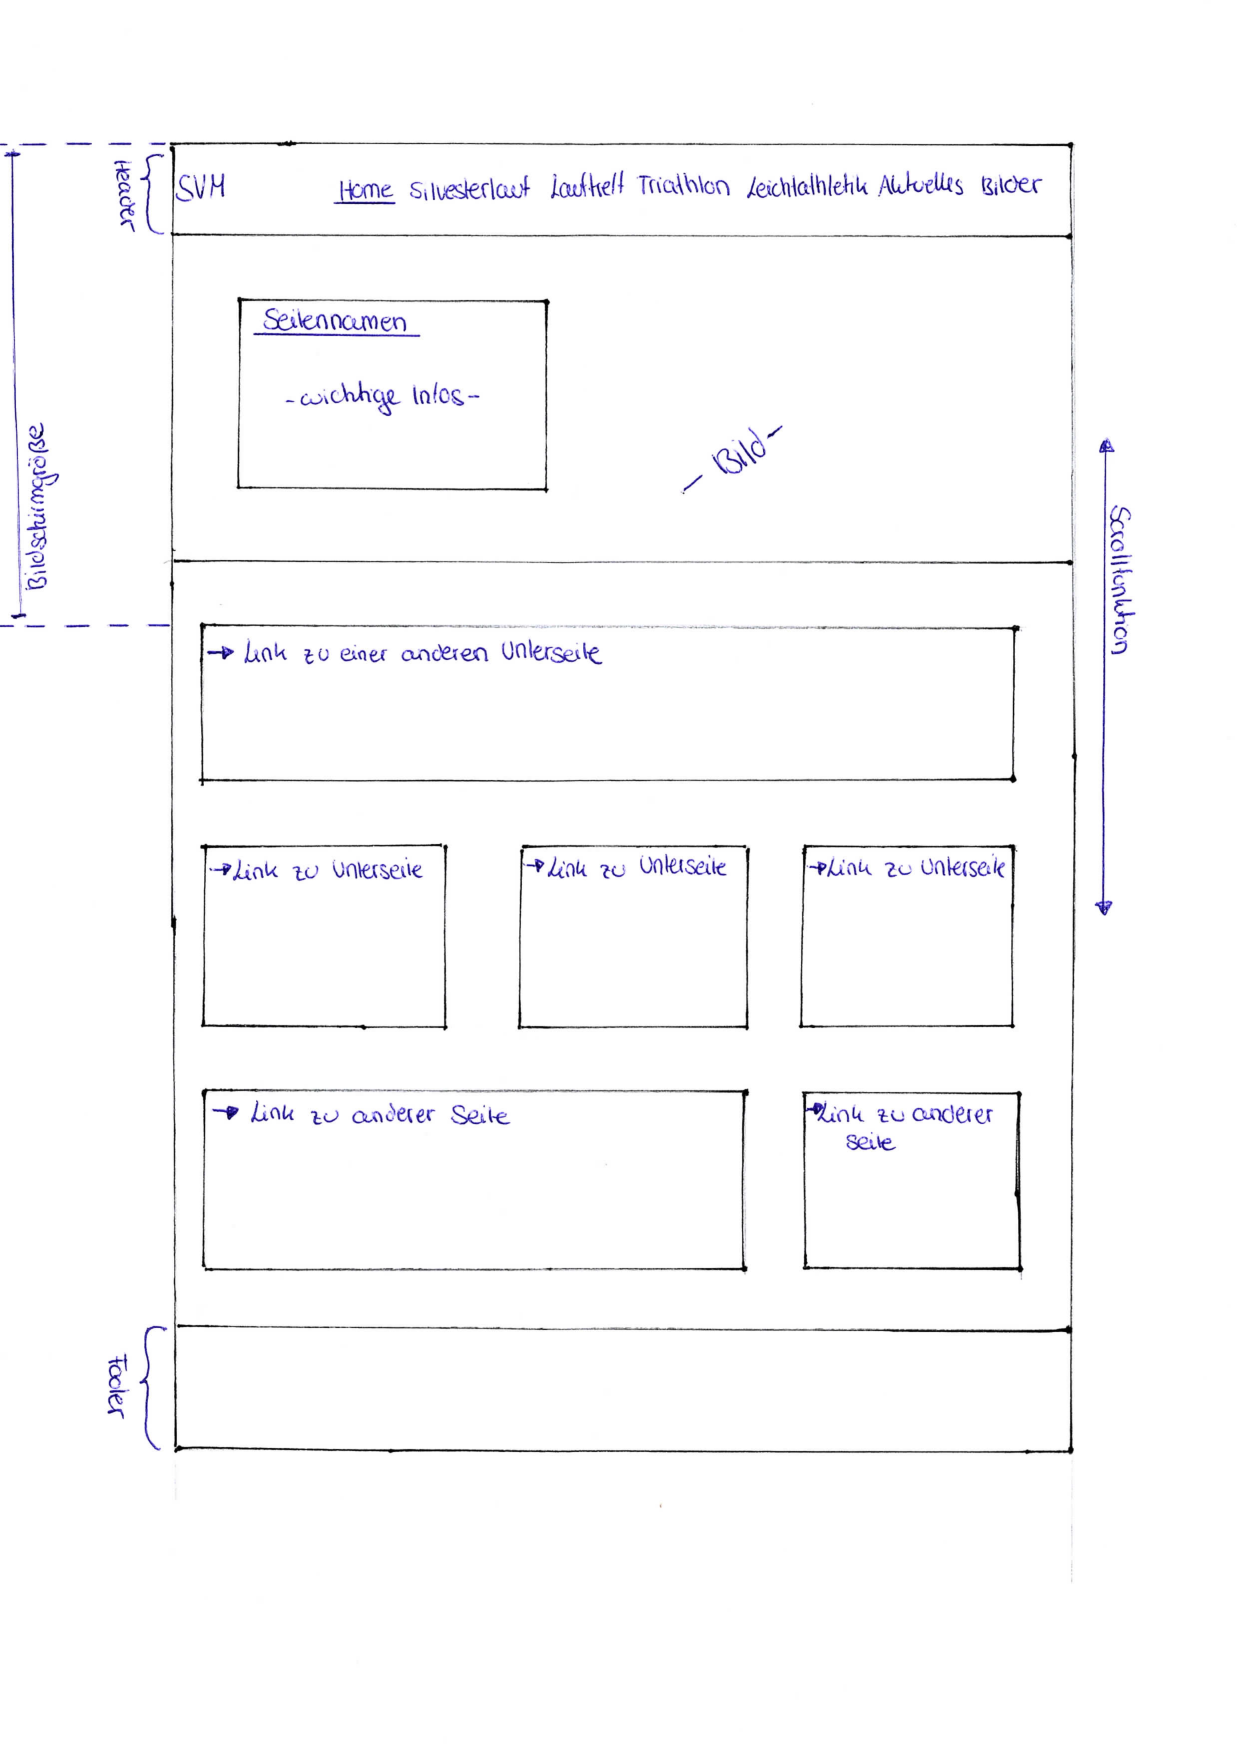
\includegraphics[scale=0.75]{Skizze01.pdf}
	\caption{Skizze1}
	\label{img:Skizze1}
\end{figure}
\newpage
\begin{figure}[!htbp]
	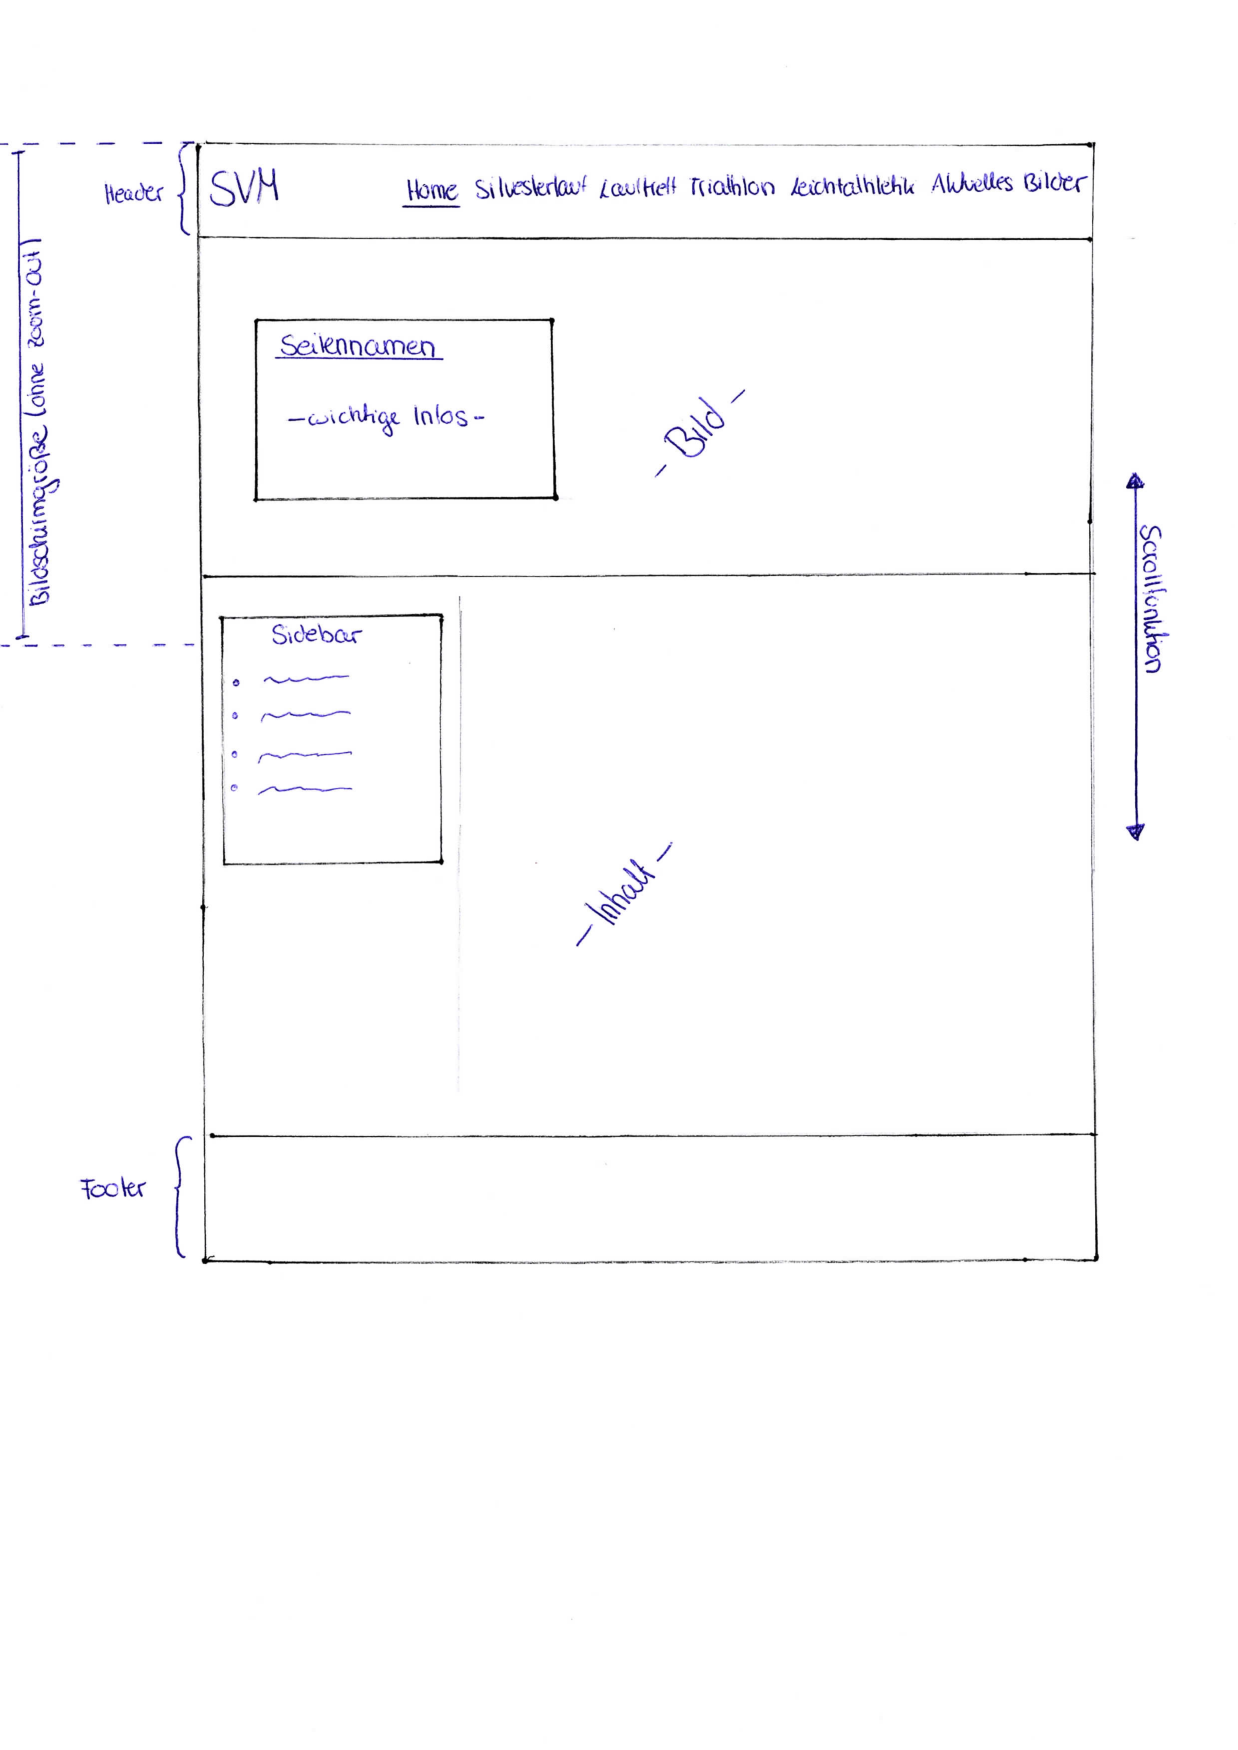
\includegraphics[scale=0.75]{Skizze02.pdf}
	\caption{Skizze2}
	\label{img:Skizze2}
\end{figure}
\newpage
\subsection{Design}
\begin{wrapfigure}{l}{7.5cm}
  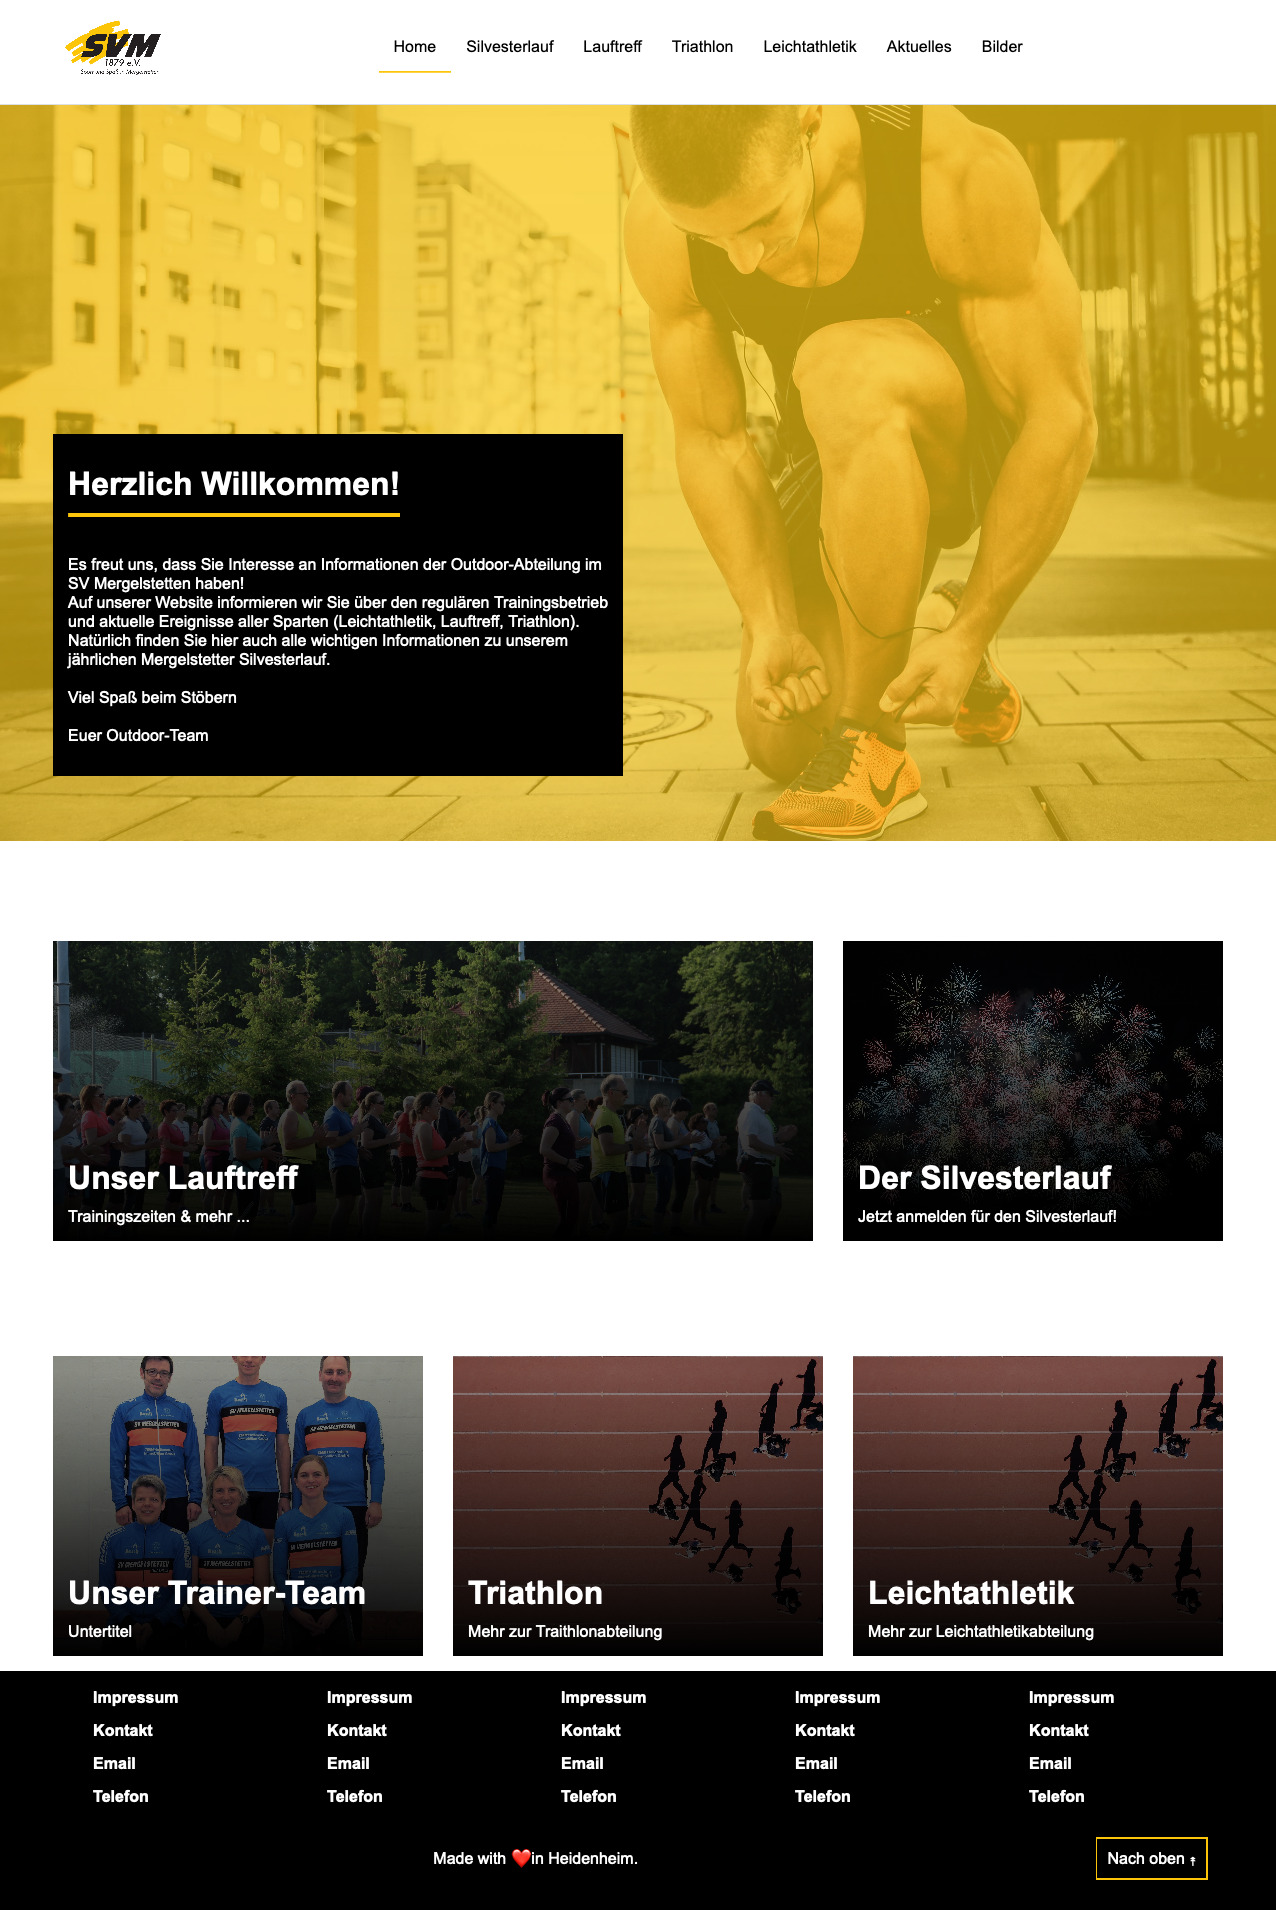
\includegraphics[width=7cm]{Home_Outdoor.jpg}
  \caption{Desktop Ansicht}
\end{wrapfigure}Bei dem Design der Webseite haben wir zu Beginn ein paar Anhaltspunkte geliefert bekommen. Beispielweise einen Pool an verschiedenen Farben oder ein Pool an verschiedenen Logos, aus dem wir uns ein paar zur Gestaltung der Webseite aussuchen können.\\
Bei der Farbgebung haben wir uns für die Vereinsfarben, also gelb, schwarz und weiß und nicht für die Outdoor-Abteilungsfarben entschieden. Wir waren uns relativ schnell einig, dass es im Hinblick darauf, dass die Website \dq Outdoor\dq \ ein Teil der Webseite  SV Mergelstetten ist, besser ist, wenn wir uns für die Vereinsfarben entscheiden. Dies ergibt nämlich ein einheitliches Gesamterscheinungsbild der später zusammengesetzten SVM-Webseite und lässt den Bereich Outdoor nicht abgegrenzt vom Rest des Sportvereins, wirken.\\
Auch bei der Auswahl des Logos haben wir uns an der vorhandenen SVM-Webseite orientiert und uns somit das vektorisierte Logo mit gelbem Wischer und Text entschieden. Zudem erschien uns dieses Logo einfach farbenfroher, ansprechender und aufgrund der Tatsache, dass es auch das Vereinsgelb in sich trägt, passender zu unserer ausgewählten Farbgebung.
Im Gegensatz zu der Farbgebung und dem Logo standen uns bei der Auswahl der Schriftart keine Anhaltspunkte zur Verfügung. Dementsprechend haben wir uns anhand anderer Auswahlkriterien entschieden. \\
 IT-Systeme wie Browser stellen nämlich nicht alle die gleichen Schriftarten bereit. Folge davon ist, dass Alternativschriftarten (z.B.: aus der gleichen Schriftfamilie) verwendet werden, Schriftarten nachgeladen werden müssen oder das Design von Anfang an nur die immer vorhandenen Schriftarten beinhalten muss.\\
Damit keine Schriften nachgeladen werden müssen, haben wir das Problem wie folgt gelöst: Unsere sogenannte Font-family beinhaltet die Arial, Helvetica, sans-serif.  Die Font-Family beschreibt hier, dass der Browser die erste Schrift der Auswahlliste benutzen wird, die er auch bereitstellt. In unserer Liste haben wir Schriften aufgezählt, die für uns optisch am ansprechendsten und gleichzeitig
gut lesbar sind. Arial ist zudem eine Schriftart, die im Normalfall bei jedem IT-System vorhanden ist, somit werden unsere Alternativschriftarten voraussichtlich kaum zum Einsatz kommen.

\subsection{Statisch - unser Verständnis}
Unter statisch verstehen wir die Bereitstellung von vorher erstellten Dateien auf einem Webserver. Für jeden Besucher sind also alle Inhalte gleich. Um Änderungen durchzuführen müssen die auf dem Webserver bereitgestellten Dateien geändert werden.
\subsection{Seitenaufbau}
Jede Unterseite unserer Website hat grundlegend den selben Aufbau, den wir uns vorher klar definiert haben, um Einheitlichkeit zu schaffen. Die einzelnen Bestandteile werden nachfolgend kurz erklärt.
\subsubsection{Header}
In der Kopfzeile, dem sogenannten \textit{Header}, hat jeder Besucher der Webseite die Möglichkeit zwischen den Unterseiten zu navigieren.\\
Ganz links findet sich als kleines Bild das Logo des Vereins wieder.
\subsubsection{Hero}
Der \textit{Hero} ist das jeweilige Titelbild jeder Unterseite. Hier bekommt der Besucher den wichtigen ersten Eindruck der Seite.\\
Innerhalb dieses Heros bekommt der Besucher außerdem direkt erste Informationen und wichtige Fakten, Links und Termine angezeigt.\\
\subsubsection{Inhaltsbereich}
Jeder \textit{Inhaltsbereich} der Seiten gliedert sich gleich in
Sidebar und Text.
\paragraph{Sidebar}
Hier werden immer kurz die Überpunkte der jeweiligen Seite dargestellt, um eine Navigation auf der Seite zu ermöglichen.
\paragraph{Text}
Hier wird der jeweilige vorgegebene Text aufgearbeitet und dargestellt. Auch Tabellen und Listen finden hier Platz.
\subsubsection{Footer}
In der Fußzeile, dem \textit{Footer}, finden sich Links zum Impressum und zur Datenschutzerklärung, sowie Links zu den Unterseiten unserer Webseite. Er ist schlicht mit weißer Schrift auf schwarzem Hintergrund gehalten und bietet dem Besucher außerdem die Möglichkeit direkt zum Anfang der Seite zu springen.
\section{"Werkzeugkasten"}
In unserem sogenannten \textit{Werkzeugkasten} \emph{(elements.html)} definieren wir unsere Grundbausteine der Webseiten, von denen einige hier kurz näher beleuchtet werden sollen. Wir haben einen solchen erstellt, um Einheitlichkeit, wie bereits oben genannt, zu schaffen und um den Einsteigern in unserer Gruppe das Arbeiten mit HTML zu erleichtern.
\paragraph{Container}
Jeder Content, egal ob Text im Hero, Text, Sidebar, Inhalt des Headers oder des Footer, wird immer in einen sogenannten \textit{Container} gepackt.
Ein solcher Container ist immer maximal 1200 Pixel breit. So erreichen wir ein einheitliches und aufgeräumtes Erscheinungsbild der Webseite.
\paragraph{Text}
Wir haben uns entschieden den \textit{Text} und die Sidebar in einem dreigeteilten Grid  anzuordnen. Ein Grid kann man sich hierbei als Gitter, beziehungsweise Tabelle, vorstellen  bei dem Teile für bestimmte Inhalte reserviert sind. Der Text nimmt hierbei die letzten, rechten zwei Drittel ein.
\paragraph{Sidebar}
Die \textit{Sidebar} ist, wie bereits im Kapitel drei beschrieben, für die Navigation auf der Seite selbst zuständig. Angezeigt wird sie immer im ersten, linken Drittel des oben genannten Grids.
\paragraph{Buttons}
Bei den \textit{Buttons} haben wir uns für vier verschiedene Varianten entschieden, die alle im Einklang mit dem sonstigen Design, beziehungsweise mit der Farbgebung der Webseite, sind.
\begin{enumerate}
\item{Komplett gelber Button mit schwarzem Text}
\item{Weißer Button mit gelbem Rand}
\item{Weißer Button mit schwarzem Rand}
\item{Komplett schwarzer Button mit weißem Text}
\end{enumerate}
\paragraph{(Werbe-)Blöcke}
Auch dieser Baustein ist in einem Grid definiert, das jedoch einen Mindestabstand von 30 Pixel zwischen den Elementen fordert. Hier ist aber die Aufteilung dynamisch. Werden also beispielsweise vier solche Blöcke eingebaut, nimmt jeder davon ein Viertel der Breite abzüglich des Mindestabstands ein.
\section{Entwicklung}
\subsection{Eingesetzte Technologien}
\subsubsection{Server}
Für die serverseitige Software haben wir uns bewusst gegen XAMPP entschieden, und uns für den Server ExpressJS\footnote{\label{foot:1} http://expressjs.com/de} entschieden. Gründe hierfür waren unter anderem die weitaus einfachere, einheitliche Konfiguration in einer Datei, welche von den Teammitgliedern nicht geändert werden muss und die erheblich höhere Antwortgeschwindigkeit.
\subsubsection{Git und GitHub}
Um effizient und koordiniert in einer Gruppe ein Softwareprodukt entwickeln zu können, haben wir Git bzw. den Dienstleister GitHub\footnote{\label{foot:2} http://github.com} als Softwaretool in den Entwicklungsprozess aufgenommen.\\
Git ermöglicht es, Zwischenstände von Quellcode einer Software zu speichern und dezentral auf einem oder mehreren Servern anderen Teilnehmern den Zugang zu ermöglichen, während auf dem lokalen Gerät weitergearbeitet werden kann.\\
Die Software nutzt dafür sogenannten \textit{Commits} (Zwischenstände) welche manuell vom Nutzer auf einem sogenannten \textit{Branch} erstellt werden. \\
Ein \textit{Branch} kann dabei als Arbeitsumgebung bzw. Zeitstrahl eines Nutzers verstanden werden, welcher mit einem eindeutigen Namen versehen ist. Dieser enthält jeweils eine Kopie des Gesamtprojektes.
Git ermöglicht es, jederzeit zu einem vorherigen Stand zurückzukehren, falls die Entwicklung in eine falsche Richtung gegangen ist oder ein Teil unabsichtlich gelöscht oder geändert wurde.\\
GitHub erweitert Git um weitere Funktionen und ermöglicht eine Partizipation aller Gruppenmitglieder durch die Möglichkeit der Erstellung von Anmerkungen, Kommentaren und Verbesserungsvorschlägen. 
\begin{figure}[!htbp]
	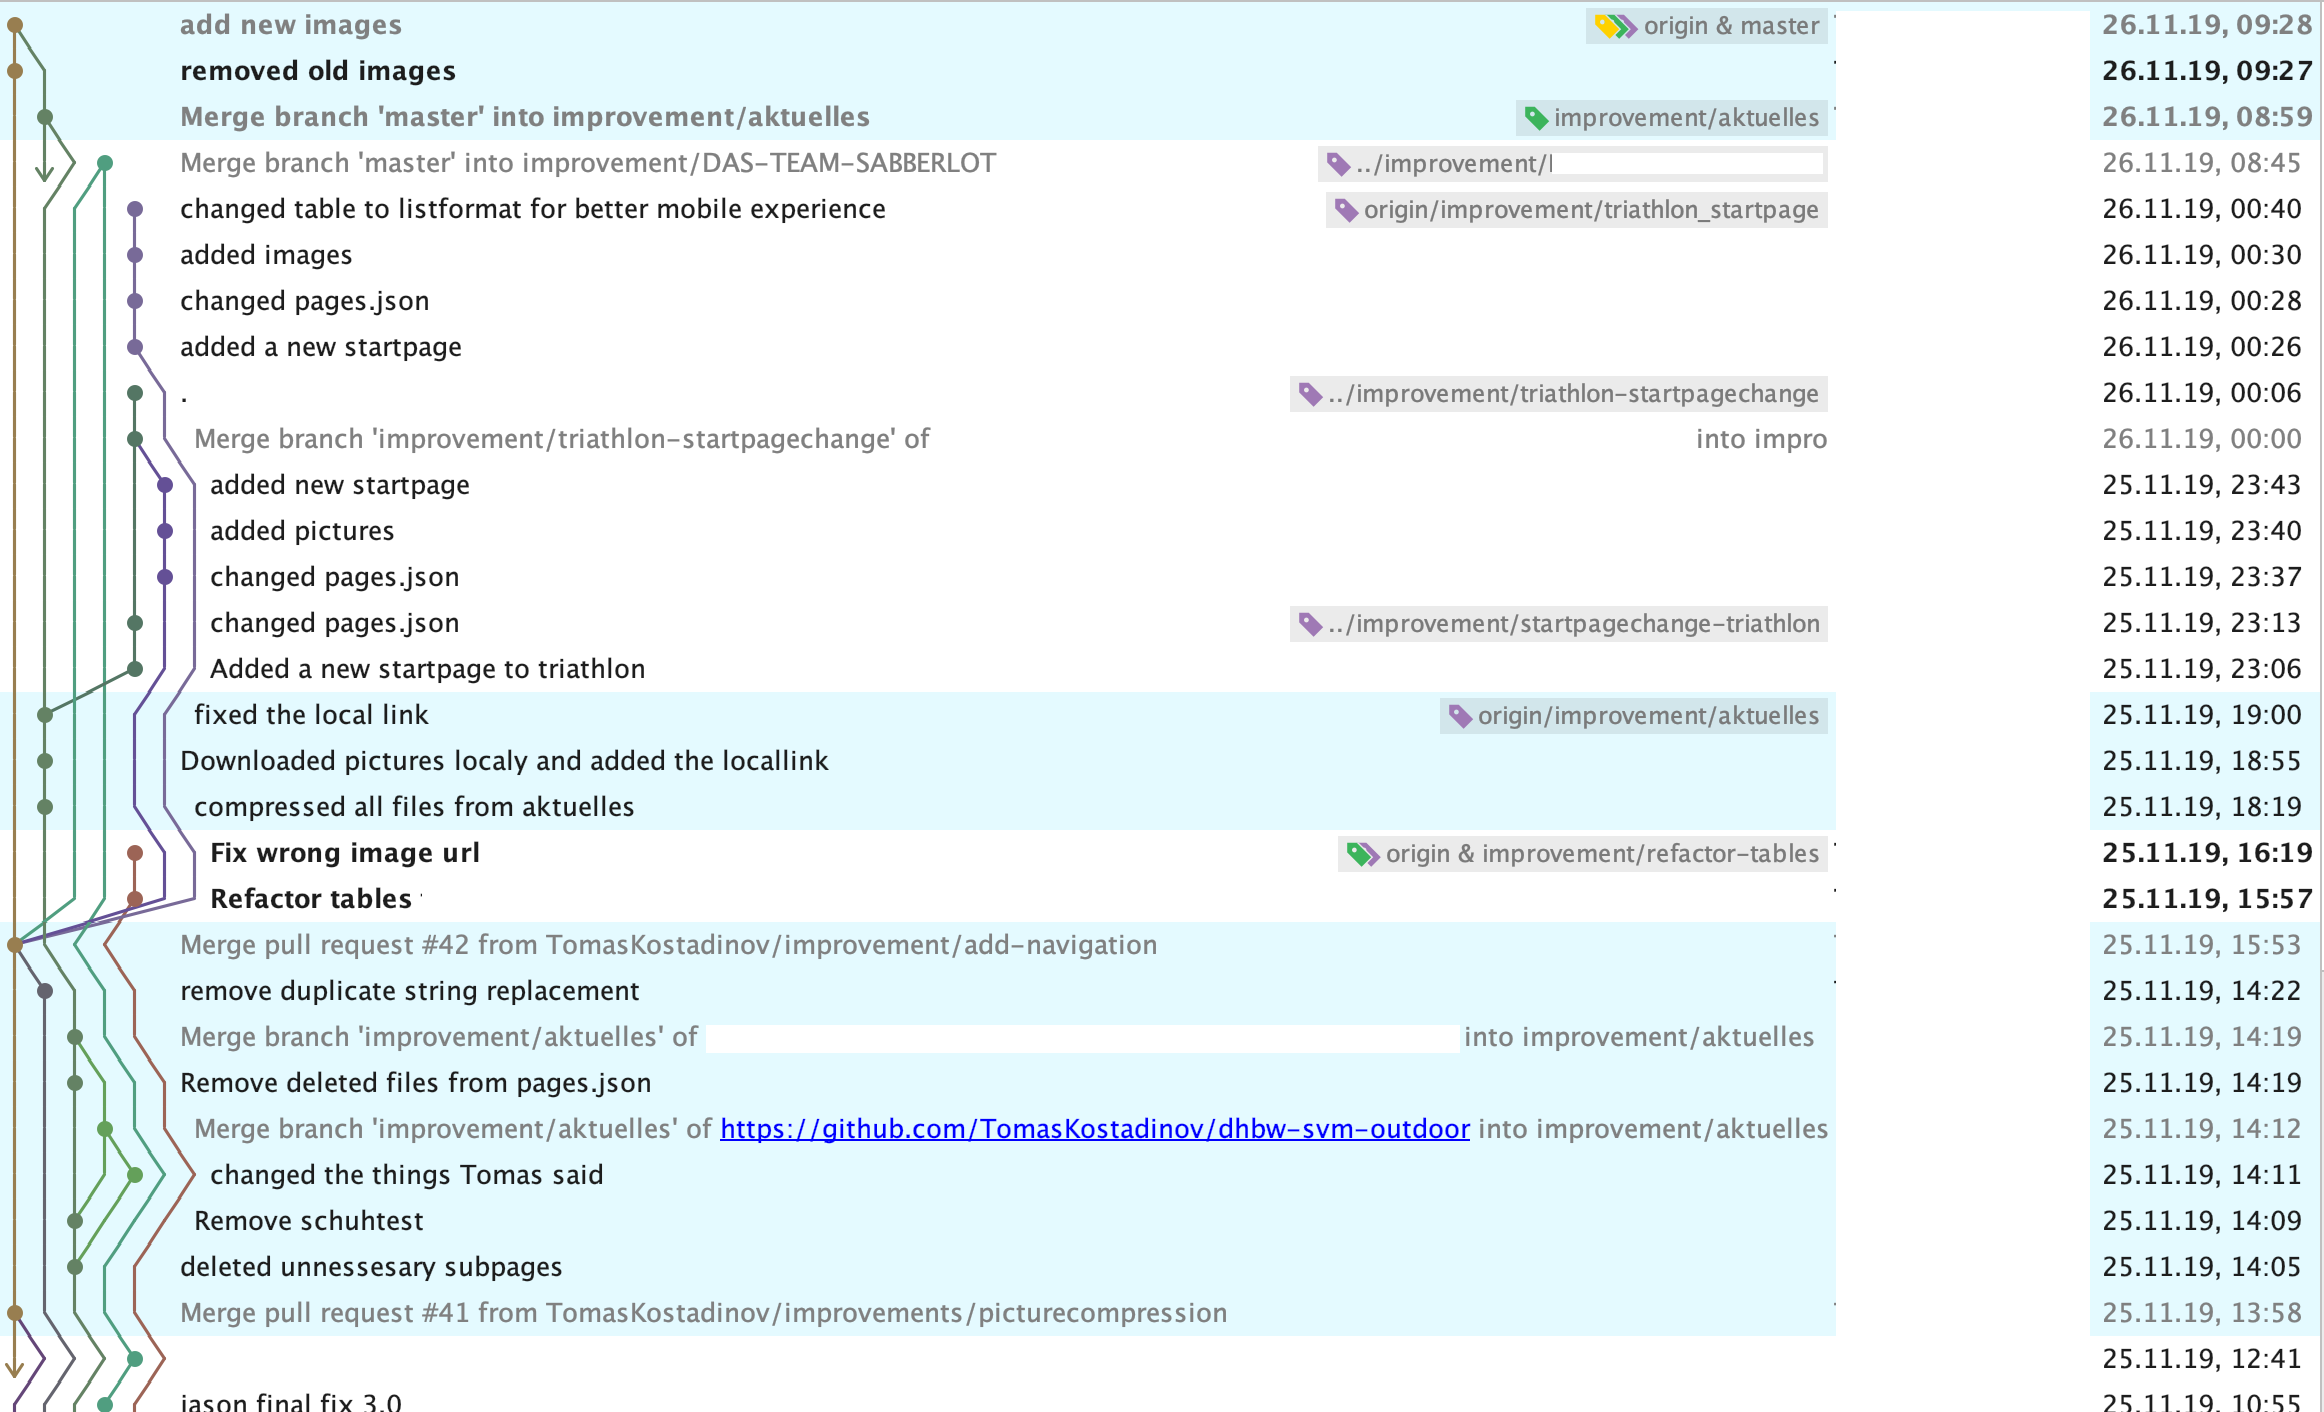
\includegraphics[scale=0.4]{git.png}
	\caption{Git - Der Entwicklungsverlauf des Projektes, wobei Branches als Linie und Commits als Punkt/Zeile dargestellt wurden.}
	\label{img:git}
\end{figure}
\subsubsection{Deployment}
Um die Entwicklung zu vereinheitlichen und schnell sichtbare Ergebnisse zu liefern, haben wir uns dafür entschieden, automatisches Deployment mit Heroku\footnote{\label{foot:3} https://heroku.com} zu integrieren.\\
Dabei wird der jeweils aktuellste Stand des Projektes isoliert und automatisiert auf einem eigenen virtuellen Server bereitgestellt. Für jeden Branch, für den ein Pullrequest (siehe weiter unten) angelegt wurde, wird ebenfalls automatisch ein neuer virtueller Server aufgesetzt. So können klar abgegrenzt jeweils die Änderungen kontrolliert werden, ohne jeweils den Quellcode lokal herunterladen und ausführen zu müssen.

\subsection{Entwicklungsprozess}
Der Entwicklungsprozess lief, bestimmt von Git, dabei folgendermaßen ab:
\subsubsection{Planung}
Das Feature, welches umgesetzt werden soll, wurde durch die Gruppe geplant und ein Verantwortlicher mit der Umsetzung beauftragt. \\
\emph{Beispiel: Teammitglied A wird durch die Gruppe beauftragt, die Triathlonunterseite zu implementieren.}
\subsubsection{Umsetzung}
Der für die Umsetzung Verantwortliche erstellt das neue Feature auf einer eigenen Kopie des master-Branchs (Anmerkung: Der sog. master ist standartmäßig der erste Branch. Er enthält den aktuellsten, fertigen Quellcode).\\
Zur Überprüfung wird der Server lokal ausgeführt und visuell das Ergebnis des Codes angeschaut.\\
Nach Erstellung und Fertigstellung wird der Stand durch den Verantwortlichen committed und auf GitHub hochgeladen (sog. push). 
\emph{Beispiel: Teammitglied A setzt die Triathlonunterseite in HTML und CSS um, committed sie auf dem Branch \textbf{improvement/add-triathlon} und pusht sie auf den Server.}
\subsubsection{Überprüfung}
Um das neue Feature in den master-Branch einzufügen, muss ein Pullrequest auf GitHub erstellt werden. Bei diesem gibt der Ersteller desselben an, welche Teile des Projekts warum geändert wurden (Bsp. Vorher-Nachher Screenshot). \\
\emph{Beispiel: Teammitglied A erstellt einen Pullrequest von \textbf{improvement/add-triathlon} nach master. Dieser Erhält automatisch eine Nummerierung (\# 34) und ein Deployment (svm-dh-pr-34.herokuapp.com).}\\
Um die Qualität des Quellcodes des Projekts sichern zu können, haben wir uns entschieden, dass zu jeder Weiterentwicklung durch ein Teammitglied ein Code Review durchgeführt werden muss. Jedes Teammitglied ist dabei berechtigt, ein Code Review abzugeben, es ist jedoch mindestens ein zustimmendes Review notwendig, um die Änderungen zu bestätigen. Der Ersteller kann dabei auch ein Teammitglied bestimmen, welches das Code Review durchführen soll.\\
\emph{Beispiel: Teammitglied A fordert ein Code Review von Teammitglied B an.}\\
Das Code Review besteht aus zwei Teilen:
\begin{enumerate}
\item{\textbf{Dem buchstäblichen Code Review}\\Dabei wird der Quellcode selbst bzw. dessen Delta (Neue/Gelöschte Zeilen) Zeile für Zeile durchgegangen und, falls notwendig, kommentiert und mit Anmerkungen versehen. Falls Änderungen notwendig sind, wird der Pullrequest temporär abgelehnt, bis diese Umgesetzt wurden.\\
\emph{Beispiel: In der Datei der Startseite der Triathlon-Mannschaft tritt ein Syntaxfehler auf. Teammitglied B bemerkt dies und fordert Änderungen an.}}
\item{\textbf{Dem visuellen Review}\\Beim visuellem Review klickt sich der Reviewer durch die neuen (und alten) Teile der Webseite auf dem Deployment des Pullrequests. Falls es auf diesem visuelle Probleme gibt, merkt der Reviewer dies in dem zugehörigen Pullrequest an und lehnt diesen ebenfalls temporär ab.\\
\emph{Beispiel: Eine Bilddatei wird trotz korrekter Syntax nicht geladen. Teammitglied B bemerkt dies und fordert von A Änderungen an.}}
\end{enumerate}
Wenn alle angemerkten und geforderten Änderungen gemacht – oder etwa keine Notwendig waren – kann der Reviewer den Status des Pullrequest auf approved setzen und so in den \textbf{master} einfügen.\\
Dieser wird dann autmatisch deployed.
\subsection{Optimierung}
Die komplette Webseite wurde darauf optimiert, auf möglichst vielen Endgeräten nutzbar zu sein. Dabei wurde auf Nutzbarkeit, Design und Geschwindigkeit geachtet (so wurden z.B. alle Bilder verlustfrei komprimiert, was zu einer Minderung der Downloadgröße um 70\% führte). Änderungen wurden direkt auf Mobil- und weiteren Endgeräten getestet, unter anderem auch auf unterschiedlichen Smartphones mit unterschiedlichen Betriebssystemen oder gar einer SmartWatch.
\begin{figure}[!htbp]
\centering
	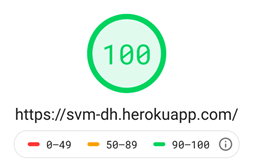
\includegraphics[scale=1]{Bewertung.png}
	\caption{Bewertung via PageSpeed Insights}
	\label{img:Bewertung}
\end{figure}
Des weiteren wurde die Webseite für Suchmaschinen wie Google optimiert. Auf dem von Google bereitgestellten Testtool \dq PageSpeed Insights\dq \footnote{\label{foot:4} https://developers.google.com/speed/pagespeed/insights} erhielt unsere Website 100 von 100 möglichen Punkten (d.h. die Bestnote, siehe Abb. 2) wobei Ladezeiten, Design und weitere Optimierungen automatisiert bewertet wurden. Zum Vergleich: die Webseite der Dualen Hochschule Heidenheim erhielt lediglich 60 von 100 Punkten. \\
Diese Bewertung ist ein großer Faktor in der Bewertung der Relevanz der Seite für Suchmaschinen und somit maßgeblich ausschlaggebend für den Listenplatz auf der Ergebnisseite. \\
Weitere Optimierungen der Website sind ein sich mit dem Hell-\/Dunkelmodus des Betriebssystems anpassender Dunkelmodus der Website und Optimierungen für eine bessere Darstellung der Website in den sozialen Netzwerken mithilfe des Open Graph Protokoll\footnote{\label{foot:5} https://developers.facebook.com/docs/sharing/webmasters}.

\section{Umsetzung}
Hier beschreiben wir die Umsetzung einzelner ausgewählter Bereiche und beantworten kurz warum was wie umgesetzt wurde.
\subsection{Team}
Da, wie bereits beschrieben, Header und Footer immer das selbe Aussehen und die selben Funktionalitäten haben, beschäftigt sich der nachfolgende Abschnitt nur mit der Umsetzung und Gestaltung der restlichen Seiten.\\
Für die Startseite haben wir uns für ein freundliches, familiäres Foto für den Hero entschieden, das den Aspekt \dq Team\dq \ unterstreicht.
Der kurze Text innerhalb des Heros zeigt dem Besucher der Webseite noch einmal kurz auf welcher Seite er sich befindet.\\
Direkt darunter folgen sieben Werbeblöcke, die per Klick zur angepriesenen Unterseite führen. Diese Unterseiten sehen dann prinzipiell immer gleich aus. Sind für einen Bereich mehrere Trainer zuständig, so erreicht man diese Unterseiten wieder über schon oben genannte Werbeblöcke, sodass jede Person eine eigene Unterseite hat.\\
Diese \dq Personenseiten\dq \ sind klassisch mit einem großen Bild und den uns vorgegeben Informationen ausgestattet.
\subsection{Aktuelles}
Bei der Seite \dq Aktuelles\dq \ spiegelt sich, mit kleinen Abweichungen, das Design der Home-Seite wieder. Das hat den Hintergrund, dass sowohl die Home-Seite als auch die Seite  \dq Aktuelles\dq \ jeweils einen Überblick verschaffen und auf weitere Unterseiten verlinken soll.\\
Auf der Grundseite \dq Aktuelles\dq \ werden Ereignisse, das neueste zuerst, aufgelistet und gleichzeitig wird ein Link zur jeweiligen Subpage, auf der dann ein Ereignis ausführlicher beschrieben wird, angegeben. Dies haben wir durch sog. Blöcke verwirklicht, wobei das aktuellste Ereignis einen größeren Block hat, sodass man dieses dadurch nicht nur besser findet, weil es oberhalb aller anderen Ereignisse steht, sondern auch dadurch, dass es größer dargestellt wird. Klickt man also auf einen Block, so gelangt man auf die Unterseite, auf der mehr Informationen zu diesem ausgewählten Anlass stehen. Das Hintergrundbild  eines solchen Blocks ist jeweils passend zu dem aktuellen Ereignis gewählt.\\
Folglich besteht unsere Seite \dq Aktuelles\dq \ aus einer Grundseite und vielen weiteren Unterseiten.\\
Bei den Unterseiten haben wir im Vergleich zu den Seiten die auch im Header verlinkt sind, den schmalen \dq Hero\dq \ benutzt, weil sich die Unterseiten so besser von der Grundseite unterscheiden lassen, und es optisch besser aussieht, da die meisten Unterseiten wenig Inhalt haben.

\subsection{Triathlon}
Auch hier war natürlich die Grundstruktur der Seiten und ihrer Unterseiten durch unsere vorherige Absprechen vorgegeben. Man musste sich also nur überlegen, wie der Inhalt strukturiert werden kann. Die Entscheidung ist dabei auf eine Aufteilung in Unterseiten pro Disziplin gefallen. Eine weitere Unterseite gibt es außerdem für Allgemeines. \\
Zu Beginn gab es noch Überlegungen ein Submenü für die Navigation zu den Unterseiten einzubinden. Schlussendlich fiel aber die Entscheidung, um im Einklang mit der restlichen Webseite zu bleiben, gegen diese Überlegung und für eine Verlinkung durch Werbeblöcke. \\
Nun fehlte nur noch die Einbindung der Informationen zu den Trainern pro Disziplin, die mit Hilfe eines Grids eingebunden wurden. \\
Damit waren die Strukturen klar und es mussten nur noch Inhalte und Links eingebunden, beziehungsweise umgesetzt, werden. 
\newpage
\section{Änderbarkeit und Wartungsfähigkeit}
Um dies bereits im statischen Ansatz möglichst gut umgesetzt zu haben, haben wir den Code soweit nur möglich kommentiert.\\
\begin{figure}[!htbp]
	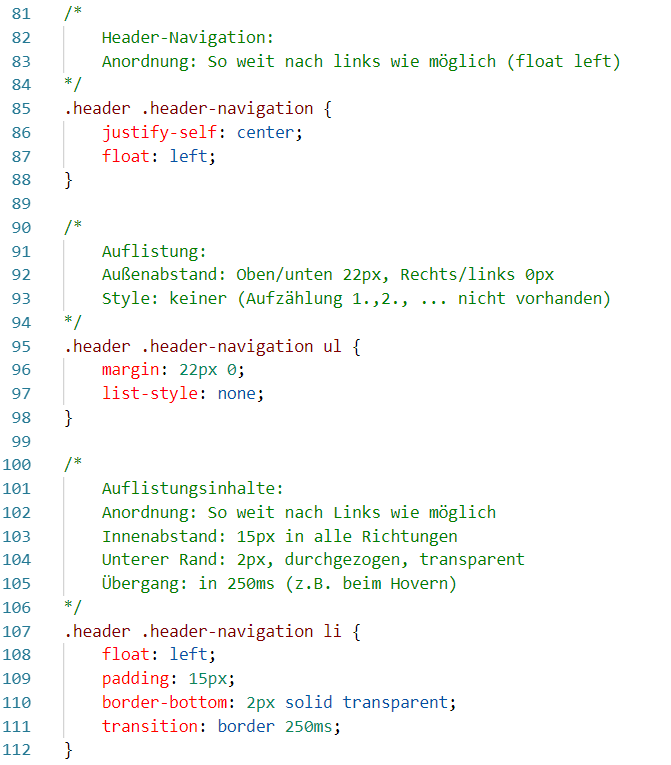
\includegraphics[scale=1.1]{Kommentierung.png}
	\caption{Kommentierung}
	\label{img:Kommentierung}
\end{figure}\\
So finden sich auch Einsteiger und Programmierunerfahrene zurecht und können kleine Änderungen durchführen. Selbst bei vollständiger Kommentierung ist es jedoch ratsam, dass Änderungen und Wartungen nur von erfahrenen Programmierern durchgeführt werden.
\newpage
\section{Funktionalität und Nutzerfreundlichkeit}
\begin{wrapfigure}{r}{9.5cm}
  
\includegraphics[width=9cm]{Home_Desktop.jpg}
  \caption{Webseitenansicht}
\end{wrapfigure}
Natürlich mussten wir unsere Webseite und damit auch alle Unterseiten auf ihre Funktionalität überprüfen. Dies erfolgte zu einem Großteil schon im vorher beschriebenen Review (Kapitel 5.1.2), jedoch konnten wir natürlich nicht garantieren, dass hier nicht doch Fehler übersehen wurden, oder Dinge doch nicht so funktionieren, wie sie sollen.\\
Um Fehler weiter zu minimieren haben wir also unsere Freunde, Bekannte, Familie und auch unsere Kommilitonen um eine Durchsicht unserer Webseite gebeten und dort entdeckte Fehler ausgebessert.\\
Den gesamten geforderten Funktionsumfang konnten wir natürlich nicht mit unserem statischen Ansatz erfüllen. Hierzu zählt unter anderem die Änderbarkeit der Seiten über einen Login-Bereich, Anmeldefunktionen und weiteres.
\section{Fazit}
Durch die regelmäßigen Treffen sind wir nie unter Zeitdruck geraten und haben keine Aufgabe aus den Augen verloren oder weniger beachtet als andere. Der Lerneffekt, den wir uns durch unser Vorgehen versprochen haben, ist auch zum größten Teil eingetroffen.
Die Gruppenarbeit selbst war, bis auf einige kleinere Differenzen, die bei einer Gruppengröße von sechs Personen unvermeidbar sind, sehr ergiebig und zielführend.\\
Hilfreich war dieses Projekt für beide \dq Parteien\dq \ in unserer Gruppe.\\
Die Erfahrenen konnten sich darin verbessern ihr Wissen weiterzugeben, komplizierte Sachverhalte einfach zu erklären und darzustellen ohne dabei die Komplexität zu weit herunter zu brechen. Außerdem lernte jeder sind in solchen Projekten zu entfalten und entwickelte so neue \dq Softskills\dq \ in diesem Bereich.\\
Auch die Einsteiger - hinsichtlich HTML - der Gruppe profitierten sehr durch das Projekt an sich. Auch hier war der größte Zugewinn im Bereich \dq Softskills\dq . Jedoch nur sehr knapp gefolgt von einem sehr großen Wissenszugewinn im Bereich Webdesign.\\
Wir hoffen diese Dynamik mit in die weiteren Teile dieses Projekts nehmen zu können und uns auch hier weiter zu entwickeln.\\
Wir freuen uns deshalb jetzt schon auf die Fortführung des Projekts in den nächsten Semestern.
\end{document}

